% ZHOU-SOURCE-PAGE: 146 PRINTED: 130

We'll show a proof of the first martingale using Ito's lemma in the next section. A
sketch for the exponential martingale is the following:\footnotemark[2]

\[
\begin{aligned}
\E[Z(t+s)]
 &=\E\left[\exp\left\{\lambda\bigl(W(t)+W(s)\bigr)-\frac{1}{2}\lambda^2(t+s)\right\}\right]\\
 &=\exp\left\{\lambda W(t)-\frac{1}{2}\lambda^2t\right\}
   \exp\left\{-\frac{1}{2}\lambda^2s\right\}
   \E\left[\exp\{\lambda W(s)\}\right]\\
 &=Z_t\exp\left\{-\frac{1}{2}\lambda^2s\right\}
   \exp\left\{\frac{1}{2}\lambda^2s\right\}=Z_t.
\end{aligned}
\]

\begin{problem}{B. What is the correlation of a Brownian motion and its square?}
\end{problem}

\begin{solution}
The solution to this problem is surprisingly simple. At time $t$, $B_t\sim N(0,t)$, by
symmetry, $\E[B_t]=0$ and $\E[B_t^3]=0$. Applying the equation for covariance
$\operatorname{cov}(X,Y)=\E[XY]-\E[X]\E[Y]$, we have
$\operatorname{cov}(B_t,B_t^2)=\E[B_t^3]-\E[B_t]\E[B_t^2]=0-0=0$.
So the correlation of a Brownian motion and its square is 0, too.

\end{solution}

\begin{problem}{C. Let $B_t$ be a Brownian motion. What is the probability that $B_1>0$ and
$B_2<0$?}
\end{problem}

\begin{solution}
A standard solution takes advantage of the fact that $B_1\sim N(0,1)$, and $B_2-B_1$
is independent of $B_1$, which is again a normal distribution: $B_2-B_1\sim N(0,1)$.
If $B_1=x>0$, then for $B_2<0$, we must have $B_2-B_1<-x$.

\[
\begin{aligned}
P(B_1>0,B_2<0)
 &=P(B_1>0,B_2-B_1<-B_1)\\
 &=\int_{\substack{x>0\\y<-x}}
   \frac{1}{\sqrt{2\pi}}e^{-x^2/2}
   \frac{1}{\sqrt{2\pi}}e^{-y^2/2}\,\dd y\,\dd x\\
 &=\int_{\substack{x>0\\y<-x}}
   \frac{1}{2\pi}e^{-(x^2+y^2)/2}\,\dd y\,\dd x\\
 &=\int_{\substack{3\pi/2\le\theta\le7\pi/4\\r\ge0}}
   \frac{1}{2\pi}e^{-r^2/2}r\,\dd r\,\dd\theta\\
 &=\frac{(7/4)\pi-(3/2)\pi}{2\pi}
   \left[-e^{-r^2/2}\right]_0^\infty=\frac{1}{8}.
\end{aligned}
\]

But do we really need the integration step? If we fully take advantage of the facts that
$B_1$ and $B_2-B_1$ are two IID $N(0,1)$, the answer is no. Using conditional
probability and independence, we can reformulate the equation as

\[
\begin{aligned}
P(B_1>0,B_2<0)
 &=P(B_1>0)P(B_2-B_1<0)P\bigl(\lvert B_2-B_1\rvert>\lvert B_1\rvert\bigr)\\
 &=1/2\cdot1/2\cdot1/2=1/8.
\end{aligned}
\]

\footnotetext[2]{$W(s)\sim N(0,s)$. So $\E[\exp\{\lambda W(s)\}]$ is the moment
generating function of normal random variable $N(0,s)$.}

% ZHOU-SOURCE-PAGE: 147 PRINTED: 131

This approach is better demonstrated in Figure 5.10. When we have $B_1>0$ and
$B_2-B_1<-B_1$, which accounts for $1/8$ of the density volume. (All 8 regions
separated by $x=0$, $y=0$, $y=x$, and $y=-x$ have the same density volume by symmetry.)

\begin{figure}[H]
  \centering
  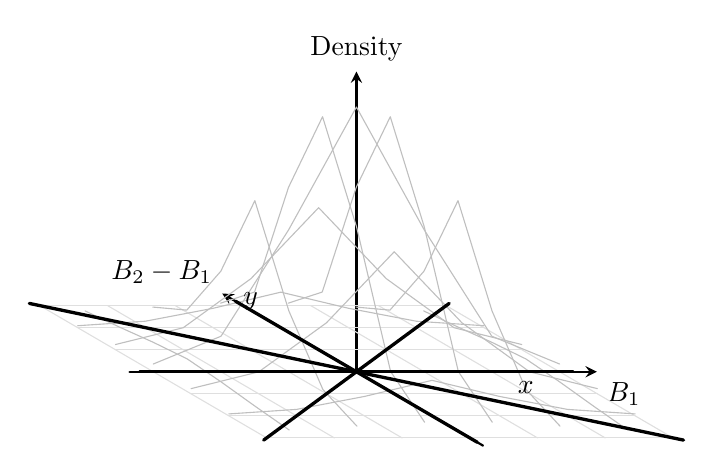
\begin{tikzpicture}[x={(0.86cm,0cm)},y={(-0.48cm,0.28cm)},z={(0cm,0.82cm)},
    >=stealth,line cap=round,line join=round]
    % Native perspective rendition of the independent normal-density hill.
    \draw[->,thick] (-3.35,0,0) -- (3.55,0,0) node[below right] {$B_1$};
    \draw[->,thick] (0,-3.35,0) -- (0,3.55,0) node[above left] {$B_2-B_1$};
    \draw[->,thick] (0,0,0) -- (0,0,4.65) node[above] {Density};
    \foreach \x in {-3,-2,-1,1,2,3}
      \draw[gray!25] (\x,-3,0) -- (\x,3,0);
    \foreach \y in {-3,-2,-1,1,2,3}
      \draw[gray!25] (-3,\y,0) -- (3,\y,0);
    % Mesh lines on the bell-shaped density surface.
    \draw[gray!50] plot coordinates {
      (-3,-2,0.03) (-2,-2,0.10) (-1,-2,0.30) (0,-2,0.55)
      (1,-2,0.30) (2,-2,0.10) (3,-2,0.03)};
    \draw[gray!50] plot coordinates {
      (-3,-1,0.08) (-2,-1,0.34) (-1,-1,1.10) (0,-1,2.20)
      (1,-1,1.10) (2,-1,0.34) (3,-1,0.08)};
    \draw[gray!50] plot coordinates {
      (-3,0,0.12) (-2,0,0.55) (-1,0,2.20) (0,0,4.10)
      (1,0,2.20) (2,0,0.55) (3,0,0.12)};
    \draw[gray!50] plot coordinates {
      (-3,1,0.08) (-2,1,0.34) (-1,1,1.10) (0,1,2.20)
      (1,1,1.10) (2,1,0.34) (3,1,0.08)};
    \draw[gray!50] plot coordinates {
      (-3,2,0.03) (-2,2,0.10) (-1,2,0.30) (0,2,0.55)
      (1,2,0.30) (2,2,0.10) (3,2,0.03)};
    \draw[gray!50] plot coordinates {
      (-2.5,-2.7,0.02) (-2.5,-1.8,0.08) (-2.5,-0.9,0.15)
      (-2.5,0,0.20) (-2.5,0.9,0.15) (-2.5,1.8,0.08) (-2.5,2.7,0.02)};
    \draw[gray!50] plot coordinates {
      (-1.5,-2.7,0.08) (-1.5,-1.8,0.34) (-1.5,-0.9,1.25)
      (-1.5,0,2.65) (-1.5,0.9,1.25) (-1.5,1.8,0.34) (-1.5,2.7,0.08)};
    \draw[gray!50] plot coordinates {
      (-0.5,-2.7,0.14) (-0.5,-1.8,0.62) (-0.5,-0.9,2.55)
      (-0.5,0,3.95) (-0.5,0.9,2.55) (-0.5,1.8,0.62) (-0.5,2.7,0.14)};
    \draw[gray!50] plot coordinates {
      (0.5,-2.7,0.14) (0.5,-1.8,0.62) (0.5,-0.9,2.55)
      (0.5,0,3.95) (0.5,0.9,2.55) (0.5,1.8,0.62) (0.5,2.7,0.14)};
    \draw[gray!50] plot coordinates {
      (1.5,-2.7,0.08) (1.5,-1.8,0.34) (1.5,-0.9,1.25)
      (1.5,0,2.65) (1.5,0.9,1.25) (1.5,1.8,0.34) (1.5,2.7,0.08)};
    \draw[gray!50] plot coordinates {
      (2.5,-2.7,0.02) (2.5,-1.8,0.08) (2.5,-0.9,0.15)
      (2.5,0,0.20) (2.5,0.9,0.15) (2.5,1.8,0.08) (2.5,2.7,0.02)};
    % The four symmetry separators partition the base into eight equal regions.
    \draw[very thick] (-3.2,0,0) -- (3.2,0,0);
    \draw[very thick] (0,-3.2,0) -- (0,3.2,0);
    \draw[very thick] (-3.1,-3.1,0) -- (3.1,3.1,0);
    \draw[very thick] (-3.1,3.1,0) -- (3.1,-3.1,0);
    \node[below] at (2.5,0,0) {$x$};
    \node[above left] at (0,2.35,0) {$y$};
  \end{tikzpicture}
  \caption{Probability density graph of $(B_1,B_2-B_1)$}
  \label{fig:zhou-figure-5-10}
\end{figure}
\end{solution}

\subsubsection*{Stopping time/ first passage time}

\begin{problem}{A. What is the mean of the stopping time for a Brownian motion to reach either
$-1$ or $1$?}
\end{problem}

\begin{solution}
As we have discussed, $B_t^2-t$ is martingale. It can be proved by applying Ito's
lemma:

\[
\begin{aligned}
\dd(B_t^2-t)
 &=\frac{\partial(B_t^2-t)}{\partial B_t}\,\dd B_t
   +\frac{\partial(B_t^2-t)}{\partial t}\,\dd t
   +\frac{1}{2}\frac{\partial^2(B_t^2-t)}{\partial B_t^2}\,\dd t\\
 &=2B_t\,\dd B_t-\dd t+\dd t=2B_t\,\dd B_t.
\end{aligned}
\]

So $\dd(B_t^2-t)$ has no drift term and is a martingale. Let
$T=\min\{t;B_t=1\text{ or }-1\}$. At continuous time and space, the following
property still applies: A martingale stopped at

% ZHOU-SOURCE-PAGE: 148 PRINTED: 132

a stopping time is a martingale! So $B_T^2-T$ is a martingale and
$\E[B_T^2-T]=B_0^2-0=0$.

The probability that $B_t$ hits 1 or $-1$ is 1, so $B_T^2=1\Rightarrow
\E[T]=\E[B_T^2]=1$.

\end{solution}

\begin{problem}{B. Let $W(t)$ be a standard Wiener process and $\tau_x$ ($x>0$) be the first
passage time to level $x$ ($\tau_x=\min\{t;W(t)=x\}$). What is the probability density
function of $\tau_x$ and the expected value of $\tau_x$?}
\end{problem}

\begin{solution}
This is a textbook problem that is elegantly solved using the reflection principle, so
we will simply summarize the explanation. For any Wiener process paths that reach $x$
before $t$ ($\tau_x\leq t$), they have equal probability ending above $x$ or below $x$
at time $t$, $P(\tau_x\leq t,W(t)\geq x)=P(\tau_x\leq t,W(t)\leq x)$. The explanation
lies in the reflection principle. As shown in Figure 5.11, for each path that reaches
$x$ before $t$ and is at a level $y$ above $x$ at time $t$, we can switch the sign of any
move starting from $\tau_x$ and the reflected path will end at $2x-y$ that is below $x$
at time $t$. For a standard Wiener process (Brownian motion), both paths have equal
probability.

\[
\begin{aligned}
P(\tau_x\leq t)
 &=P(\tau_x\leq t,W(t)\geq x)+P(\tau_x\leq t,W(t)\leq x)\\
 &=2P(\tau_x\leq t,W(t)\geq x)\\
 &=2P(W(t)\geq x)=2\int_x^\infty
   \frac{1}{\sqrt{2\pi t}}e^{-w^2/2t}\,\dd w.
\end{aligned}
\]

Let $v=\dfrac{w}{\sqrt{t}}$, we have $e^{-w^2/2t}=e^{-v^2/2}$ and
$\dd v=\dfrac{\dd w}{\sqrt{t}}$.

\[
\therefore\quad P(\tau_x\leq t)=2\int_x^\infty\frac{1}{\sqrt{2\pi t}}e^{-w^2/2t}\,\dd w
=2\int_{x/\sqrt{t}}^\infty\frac{1}{\sqrt{2\pi}}e^{-v^2/2}\,\dd v
=2-2N\left(\frac{x}{\sqrt{t}}\right)\,.\footnotemark[3]
\]

Take the derivative with respect to $t$, we have

\[
\begin{aligned}
f_{\tau_x}(t)&=\frac{\dd P\{\tau_x\leq t\}}{\dd t}\\
&=\frac{\dd P\{\tau_x\leq t\}}{\dd(x/\sqrt{t})}
  \frac{\dd(x/\sqrt{t})}{\dd t}\\
&=2N'\left(\frac{x}{\sqrt{t}}\right)\cdot\frac{x}{2}t^{-3/2}\\
&\Longrightarrow\frac{x e^{-x^2/2t}}{t\sqrt{2\pi}},\quad\forall x>0.
\end{aligned}
\]

From part A, it's easy to show that the expected stopping time to reach either
 $\alpha$ ($\alpha>0$) or $-\beta$ ($\beta>0$) is again $\E[N]=\alpha\beta$. The expected
first passage time to level $x$ is

\footnotetext[3]{If we define $M(t)=\max_{0\leq s\leq t}W(s)$, then
$P(\tau_x\leq t)$ if and only if $M(t)\geq x$. Taking the derivative of
$P(\tau_x\leq t)$ with respect to $x$, we can derive the probability density function
of $M(t)$.}

% ZHOU-SOURCE-PAGE: 149 PRINTED: 133

essentially the expected stopping time to reach either $x$ or $-\infty$ and
$\E[\tau_x]=x\cdot\infty=\infty$. Although we have
$P(\tau_x\leq\infty)=2-2N(x/\sqrt{\infty})=1$, the expected value of $\tau_x$ is $\infty$!

\begin{figure}[H]
  \centering
  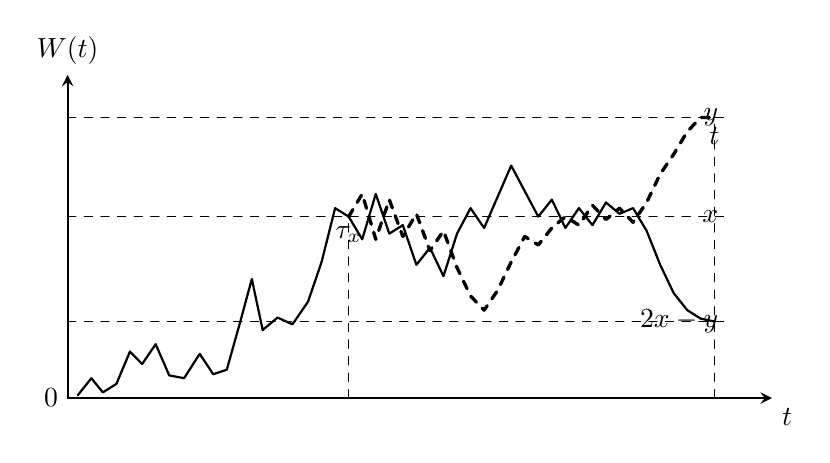
\begin{tikzpicture}[x=0.86cm,y=0.72cm,>=stealth,line cap=round,line join=round]
    \draw[->,thick] (0,0) -- (0,5.7) node[above] {$W(t)$};
    \draw[->,thick] (0,0) -- (10.4,0) node[below right] {$t$};
    \draw[dashed] (0,1.35) -- (9.75,1.35) node[left] {$2x-y$};
    \draw[dashed] (0,3.20) -- (9.75,3.20) node[left] {$x$};
    \draw[dashed] (0,4.95) -- (9.75,4.95) node[left] {$y$};
    \node[left] at (0,0) {$0$};
    \draw[dashed] (4.15,0) -- (4.15,3.20) node[below] {$\tau_x$};
    \draw[dashed] (9.55,0) -- (9.55,4.95) node[below] {$t$};
    \draw[thick] plot coordinates {
      (0.15,0.05) (0.35,0.35) (0.52,0.10) (0.72,0.25) (0.92,0.82)
      (1.10,0.60) (1.30,0.95) (1.50,0.40) (1.72,0.35) (1.95,0.78)
      (2.15,0.42) (2.35,0.50) (2.55,1.35) (2.72,2.10) (2.88,1.20)
      (3.10,1.42) (3.32,1.30) (3.55,1.70) (3.75,2.40) (3.95,3.35)
      (4.15,3.20) (4.35,2.80) (4.55,3.60) (4.75,2.90) (4.95,3.05)
      (5.15,2.35) (5.35,2.65) (5.55,2.15) (5.75,2.90) (5.95,3.35)
      (6.15,3.00) (6.35,3.55) (6.55,4.10) (6.75,3.65) (6.95,3.20)
      (7.15,3.50) (7.35,3.00) (7.55,3.35) (7.75,3.05) (7.95,3.45)
      (8.15,3.25) (8.35,3.35) (8.55,2.95) (8.75,2.35) (8.95,1.85)
      (9.15,1.55) (9.35,1.40) (9.55,1.35)};
    \draw[dashed,very thick] plot coordinates {
      (4.15,3.20) (4.35,3.60) (4.55,2.80) (4.75,3.50) (4.95,2.85)
      (5.15,3.25) (5.35,2.60) (5.55,2.95) (5.75,2.30) (5.95,1.80)
      (6.15,1.55) (6.35,1.90) (6.55,2.40) (6.75,2.85) (6.95,2.70)
      (7.15,3.00) (7.35,3.20) (7.55,3.05) (7.75,3.40) (7.95,3.15)
      (8.15,3.35) (8.35,3.10) (8.55,3.45) (8.75,3.95) (8.95,4.30)
      (9.15,4.70) (9.35,4.95) (9.55,4.95)};
  \end{tikzpicture}
  \caption{Sample path of a standard Weiner process and its reflected path}
  \label{fig:zhou-figure-5-11}
\end{figure}

\end{solution}

\begin{problem}{C. Suppose that $X$ is a Brownian motion with no drift, i.e.
$\dd X(t)=\dd W(t)$. If $X$ starts at 0, what is the probability that $X$ hits 3 before
hitting $-5$? What if $X$ has drift $m$, i.e. $\dd X(t)=m\,\dd t+\dd W(t)$?}
\end{problem}

\begin{solution}
A Brownian motion is a martingale. Let $P_3$ be the probability that the Brownian motion
hits 3 before $-5$. Since a martingale stopped at a stopping time is a martingale, we
have $3P_3+(-5)(1-P_3)=0\Rightarrow P_3=5/8$. Similar to random walk, if we have
stopping boundaries ($\alpha>0$) and $-\beta$ ($\beta>0$), the probability that it stops
at $\alpha$ instead of $-\beta$ is $p_\alpha=\beta/(\alpha+\beta)$. The expected stopping
 time to reach either $\alpha$ or $-\beta$ is again $\E[N]=\alpha\beta$.

When $X$ has drift $m$, the process is no longer a martingale. Let $P(t,x)$ be the
probability that the process hits 3 before hitting $-5$ when $X=x$ at time $t$. Although
$X$ is no longer a

% ZHOU-SOURCE-PAGE: 150 PRINTED: 134

martingale process, it is still a Markov process. So $P(t,x)=P(x)$ is actually independent
of $t$. Applying the Feynman-Kac equation\footnotemark[4], we have

\[
mP_x(x)+\frac{1}{2}P_{xx}(x)=0\qquad\text{for }-5<x<3.
\]

We also have boundary conditions that $P(3)=1$ and $P(-5)=0$.

$mP_x(x)+\frac{1}{2}P_{xx}(x)=0$ is a homogeneous linear differential equation with two
real roots: $r_1=0$ and $r_2=-2m$. So the general solution is
$P(x)=c_1e^{0x}+c_2e^{-2mx}=c_1+c_2e^{-2mx}$. Applying the boundary conditions, we
have

\[
\left\{
\begin{aligned}
c_1+c_2e^{-6m}&=1,\\
c_1+c_2e^{10m}&=0
\end{aligned}
\right.
\quad\Rightarrow\quad
\left\{
\begin{aligned}
c_1&=\frac{-e^{10m}}{e^{-6m}-e^{10m}},\\
c_2&=\frac{1}{e^{-6m}-e^{10m}}
\end{aligned}
\right.
\quad\Rightarrow\quad
P(0)=c_1+c_2=\frac{e^{10m}-1}{e^{10m}-e^{-6m}}.
\]

A different and simpler approach takes advantage of the exponential martingale:

\[
Z(t)=\exp\left\{\lambda W(t)-\frac{1}{2}\lambda^2t\right\}.
\]

Since $W(t)=X(t)-mt$, $X(t)-mt$ is a Brownian motion as well. Applying the exponential
martingale, we have
$\E\left[\exp\left\{\lambda(X-mt)-\frac{1}{2}\lambda^2t\right\}\right]=1$ for any
constant $\lambda$. To remove the terms including time $t$, we can set $\lambda=-2m$ and
the equation becomes $\E[\exp(-2mX)]=1$. Since a martingale stopped at a stopping time is
a martingale, we have

\[
P_3\exp(-2m\cdot3)+(1-P_3)\exp(-2m\cdot-5)=1
\quad\Rightarrow\quad
\frac{e^{10m}-1}{e^{10m}-e^{-6m}}.
\]

\end{solution}

\begin{problem}{D. Suppose that $X$ is a generalized Weiner process $\dd X=\dd t+\dd W(t)$, where
$W(t)$ is a Brownian motion. What is the probability that $X$ ever reaches $-1$?}
\end{problem}

\begin{solution}
To solve this problem, we again can use the equation $\E[\exp(-2mX)]=1$ from the previous
problem with $m=1$. It may not be obvious since we only have one apparent boundary, $-1$.
To apply the stopping time, we also need a corresponding positive boundary. To address this
problem, we can simply use $+\infty$ as the positive boundary and the equation becomes

\footnotetext[4]{Let $X$ be an Ito process given by equation
$\dd X(t)=\beta(t,X_t)\,\dd t+\gamma(t,X_t)\,\dd W$ and $f(x)$ be a function of $X$. Define function
$V(t,x)=\E[f(X_T)\vert X_t=x]$, then $V(t,x)$ is a martingale process that satisfies the
partial differential equation
\[
\frac{\partial V}{\partial t}+\beta(t,x)\frac{\partial V}{\partial x}
+\frac{1}{2}\gamma^2(t,x)\frac{\partial^2V}{\partial x^2}=0
\]
and terminal condition $V(T,x)=f(x)$ for all $x$.}
